\documentclass[tikz,border=3.14mm]{standalone}
\usetikzlibrary{calc}

\begin{document}
    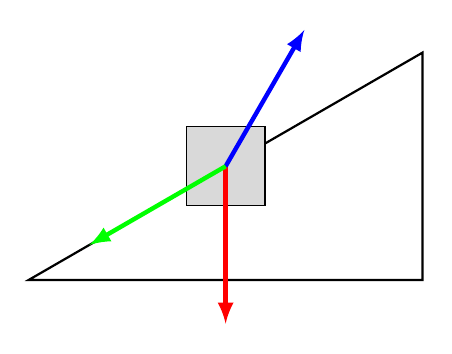
\begin{tikzpicture}
        \def\angle{30}  % Theta
        
        % Inclined Plane
        \draw[black, thick] (0,0) -- (5,0) -- (5,{5*tan(\angle)}) -- cycle;
    
        % Block
        \draw[fill=gray!30] ($(2.5,{2.5*tan(\angle)}) + (0.5, 0.5)$) rectangle +(-1,-1);
        
        % Forces
        \draw[red, -latex, ultra thick] (2.5,{2.5*tan(\angle)}) -- +(0,-2); % gravity
        \draw[blue, -latex, ultra thick] (2.5,{2.5*tan(\angle)}) -- +(90-\angle:2); % normal force
        \draw[green, -latex, ultra thick] (2.5,{2.5*tan(\angle)}) -- +(-180+\angle:2); % component of gravity along the plane
    \end{tikzpicture}
\end{document}